\subsection{Graph and its Equivalence}

    \paragraph{Execution Graph}
    
        \begin{itemize}
            \item Has all the ordering relations defined by the axiomatic model (eg: happens-before, program-order)
            \item Each execution graph is unique
        \end{itemize}
    
    
    \paragraph{Equivalence}
        \begin{center}
            \emph{\textit{
                Two execution graphs E1 and E2 are symmetric / equivalent to each other, if we can swap thread identities of one of them to form the other. 
            }}  
        \end{center}

        In terms of ordering relations, swapping thread identities means: 
        \begin{itemize}
            \item Any reads-from relation established among events of the threads being swapped are also swapped.
            \item Reads-from relation from read of a thread being swapped to an outside write is changed such that the read is that of a swapped thread having the same relation with the write.   
        \end{itemize}

        \critic{blue}{There might be other derived relations, eg: happens-before, from-reads, etc. For now we only keep it restricted to reads-from relations.}

        In short, if we tag all the thread events by some number, simply changing the numbers by their swapped thread identities will ensure the above two. 

        \critic{blue}{Note that it could be the case that an execution has two threads to be of same code, but it may not reflect what it is in the original program. The equivalence is on the assumption that both threads do have equal code in both those  executions.}

    \paragraph{Example of swapping thread identities?}
        
        %Show an example here
        \begin{figure}[H]
            \centering
            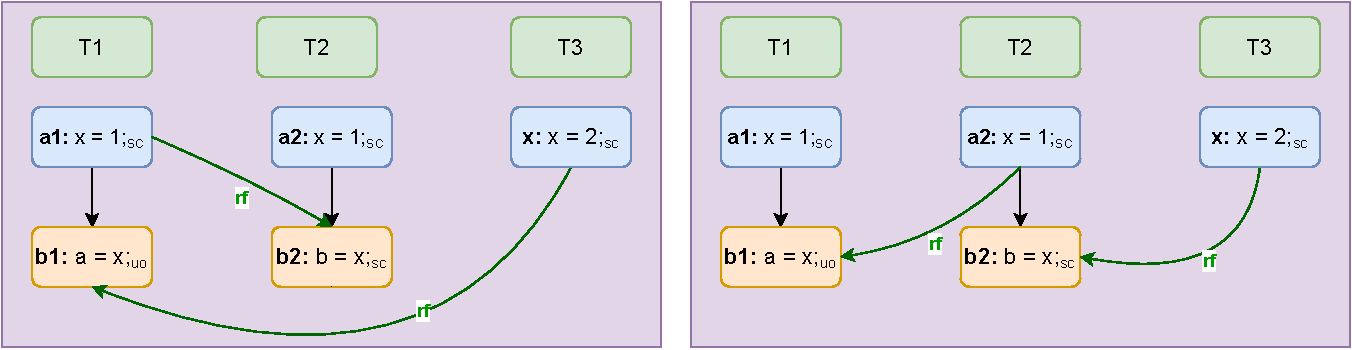
\includegraphics[scale=0.7]{Equivalence_Example.pdf}
            \caption{Example of two equivalent execution graphs}
        \end{figure}

        The two executions which are symmetric have the following reads-write relations. 
        \begin{align*}
            b1:x \ \wedge \ b2:a1 \\
            b1:a2 \ \wedge \ b2:x 
        \end{align*}

        Notice from the above figure that swapping thread identities of T1 and T2 implies jsut swapping $\{b1, b2\}$ and $\{a1, a2\}$.
        
        \critic{blue}{It took quite some time to have a clear picture of what swapping thread identities implied for us when looking at symmetric executions.}



